%% Taken from Taras answer on http://tex.stackexchange.com/questions/14901/dimensioning-of-a-technical-drawing-in-tikz


\documentclass[tikz,margin=5pt]{standalone}
\usepackage{xparse}
\usetikzlibrary{calc}

\tikzset{%
    Cote node/.style={%
        midway,
        sloped,
        fill=white,
        inner sep=1.5pt,
        outer sep=2pt
    },
    Cote arrow/.style={%
        <->,
        >=latex,
        very thin
    }
}

\makeatletter
\NewDocumentCommand{\Cote}{%
    s       % cotation avec les flèches à l'extérieur
    D<>{1.5pt} % offset des traits
    O{.75cm}    % offset de cotation
    m       % premier point
    m       % second point
    m       % étiquette
    D<>{o}  % () coordonnées -> angle
            % h -> horizontal,
            % v -> vertical
            % o or what ever -> oblique
    O{}     % parametre du tikzset
    }{%

    {\tikzset{#8}

    \coordinate (@1) at #4 ;
    \coordinate (@2) at #5 ;

    \if #7v % Cotation verticale
        \coordinate (@0) at ($($#4!.5!#5$) + (#3,0)$) ; 
        \coordinate (@4) at (@0|-@1) ;
        \coordinate (@5) at (@0|-@2) ;
    \else
    \if #7h % Cotation horizontale
        \coordinate (@0) at ($($#4!.5!#5$) + (0,#3)$) ; 
        \coordinate (@4) at (@0-|@1) ;
        \coordinate (@5) at (@0-|@2) ;
    \else % cotation encoche
    \ifnum\pdfstrcmp{\unexpanded\expandafter{\@car#7\@nil}}{(}=\z@
        \coordinate (@5) at ($#7!#3!#5$) ;
        \coordinate (@4) at ($#7!#3!#4$) ;
    \else % cotation oblique    
        \coordinate (@5) at ($#5!#3!90:#4$) ;
        \coordinate (@4) at ($#4!#3!-90:#5$) ;
    \fi\fi\fi

    \draw[very thin,shorten >= #2,shorten <= -2*#2] (@4) -- #4 ;
    \draw[very thin,shorten >= #2,shorten <= -2*#2] (@5) -- #5 ;

    \IfBooleanTF #1 {% avec étoile
    \draw[Cote arrow,-] (@4) -- (@5)
        node[Cote node] {#6\strut};
    \draw[Cote arrow,<-] (@4) -- ($(@4)!-6pt!(@5)$) ;   
    \draw[Cote arrow,<-] (@5) -- ($(@5)!-6pt!(@4)$) ;   
    }{% sans étoile
    \ifnum\pdfstrcmp{\unexpanded\expandafter{\@car#7\@nil}}{(}=\z@
        \draw[Cote arrow] (@5) to[bend right]
            node[Cote node] {#6\strut} (@4) ;
    \else
    \draw[Cote arrow] (@4) -- (@5)
        node[Cote node] {#6\strut};
    \fi
    }}
    }
\makeatother

\begin{document}
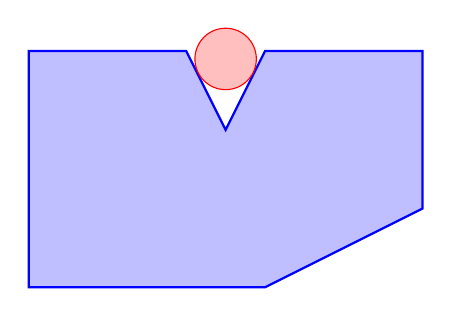
\begin{tikzpicture}
\small
\draw[thick,blue,fill=blue!25]
        (0,1) coordinate (A)
    --  (3,1) coordinate (B)
    --  (5,2) coordinate (C)
    --  (5,4) coordinate (D)
    --  (3,4) coordinate (E)
    --  (2.5,3) coordinate (F)
    --  (2,4) coordinate (G)
    --  (0,4) coordinate (H)
    --cycle ;

\draw[red,fill=red!25] (2.5,3.9) circle (.39) ;

\Cote{(A)}{(B)}{1}

\Cote{(B)}{(C)}{2}

\Cote{(B)}{(C)}{2 bis}<h>[Cote node/.append style={fill=blue!25}]

\Cote[.3cm]{(C)}{(D)}{3 bis}
\Cote[.7cm]{(C)}{(D)}{3}[Cote node/.append style={rotate=-90}]
\Cote[1.1cm]{(C)}{(D)}{3 ter}[%
                    Cote node/.append style={right,rotate=-90}]

\Cote[2cm]{(G)}{(E)}{?$^\circ$}<(F)>

\Cote*[1.2cm]{(2.11,3.9)}{(2.89,3.9)}{4}[%
    Cote node/.append style={below=-1pt,fill=blue!25}]

\Cote[-2cm]{(A)}{(2.5,4.29)}{5}<v>

\end{tikzpicture}
\end{document}  
